\chapter{Preliminaries}\label{chap:preliminaries}


In this chapter, we present the mathematical background that will be further needed to describe our work. We summarize gradient descent algorithm and neural networks and we outline how to train them. Some of this chapter's definitions we took from~\cite{Goodfellow-et-al-2016} which we also highly suggest for a reader more interested in the subject.


\section{Multivariable Calculus}
Let $f\colon\R^n\to\R$ be a function with all partial derivatives existing and being continuous. The \textit{gradient} of $f$ is
\begin{equation*}
\nabla f(\bm{a})=\left(\frac{\partial f(\bm{a})}{\partial x_1},\dots,\frac{\partial f(\bm{a})}{\partial x_n}\right).
\end{equation*}
We write $\nabla_{\bm{x}} f$ or simply $\nabla f$.
% For our purpose we can allow finitely many points where the partial derivatives do not exist -- there we can define them arbitrarily.
To compute the derivative of a composition of two or more functions \textit{chain rule} is used. Suppose $g\colon\R^m\to\R^n$ and $z=f(g(\bm{x}))$, then
\begin{equation*}
\frac{\partial z}{\partial x_i}=\sum\limits_{j=1}^n\frac{\partial z}{\partial g(\bm{x})_j}\frac{\partial g(\bm{x})_j}{\partial x_i}\quad\mathrm{or\ in\ vector\ form}\quad\nabla_{\bm{x}}z=\left(\frac{\partial g(\bm{x})}{\partial\bm{x}}\right)^\top\nabla_{g(\bm{x})}z
\end{equation*}
where $\frac{\partial g(\bm{x})}{\partial\bm{x}}$ is the Jacobian matrix.

Given a function $f\colon\R^n\to\R$ we may ask where are its local (or global) minima. For some functions, it can be computed analytically, for the most of them however the analytical solution is impossible and so a numerical method called \textit{gradient descent} is often used. We start with arbitrary point $\bm{x}\in \R{^n}$. Since gradient tells us how to change $\bm{x}$ in order to make a small improvement in $f(\bm{x})$, to minimize $f(\bm{x})$ we make a small change to $\bm{x}$ in the opposite direction:
\begin{equation*}
\bm{x}=\bm{x}-\alpha\nabla_{\bm{x}}f(\bm{x})
\end{equation*}
where $\alpha$ is the step size also called the learning rate. The step is repeated until convergence or for a certain number of iterations. Note that the algorithm does not have to converge even for convex functions such as $x^2$ since it can `jump' around $x=0$ indefinitely due to a bad value of $\alpha$.
Also if the algorithm converges we are not guaranteed to find the global minimum, we can even be arbitrary far from it. However, in machine learning, this algorithm with minor modifications is widely used usually producing good-enough results.

\section{Neural Networks}
Artificial feedforward neural network is a machine learning model capable of learning its parameters $\bm{\theta}$ such that given input $\bm{x}$ it predicts output $\bm{y}=f(\bm{x};\bm{\theta})$. The network is composed of smaller units called neurons defined as
\begin{equation*}
h_i=g\left(\sum_{j}w_{i,j}x_j\right)
\end{equation*}
where $h_i$ is the output of $i$\textsuperscript{th} neuron, $x_j$ are its inputs and $g$ is a nonlinear function such as $1/(1+e^{-x})$ or $\max(0, x)$. Usually, we group neurons into layers and therefore we write $\bm{h}=g(W\bm{x})$ where $W\in\R^{\dim(\bm{h})\times\dim(\bm{x})}$ and $g$ is applied componentwise. Simple feedforward neural network with one `hidden' layer can be seen in Figure~\ref{fig:basic_nn}. Such basic network can approximate any continuous functions if there are enough neurons in the hidden layer~\cite{HORNIK}. However, the number of neurons can be arbitrary big and empirically networks with more hidden layers usually achieve better results with the same number of neurons.

\begin{figure}
	\centering
	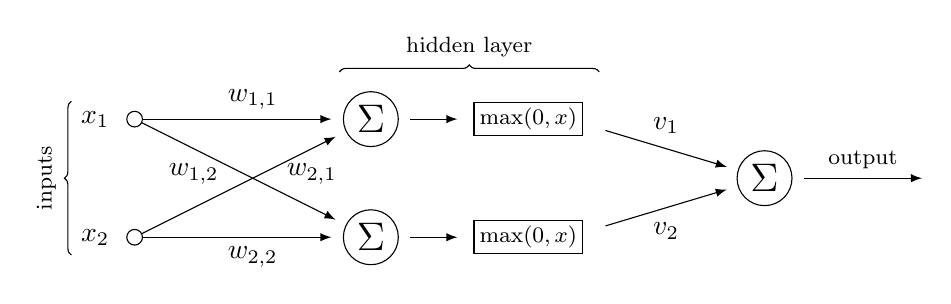
\begin{tikzpicture}[
init/.style={
	draw,
	circle,
	inner sep=2pt,
	font=\Large,
},
squa/.style={
	draw,
	inner sep=2pt,
	font=\footnotesize
}
]

\node[draw, circle, inner sep=2pt] at (0,0) {};
\node[] (x2) at (-.5,0) {$x_2$};
\draw[-latex, shorten >= 0.5cm, shorten <= 0.1cm] (0,0) -- (3,0) node[midway, below] {$w_{2,2}$};
\node[init] at (3,0) {$\displaystyle\Sigma$};
\draw[-latex, shorten >= 0.9cm, shorten <= 0.5cm] (3,0) -- (5,0);
\node[squa] at (5,0) {$\max(0,x)$};

\node[] (x1) at (-.5,1.5) {$x_1$};
\node[draw, circle, inner sep=2pt] at (0,1.5) {};
\draw[-latex, shorten >= 0.5cm, shorten <= 0.1cm] (0,1.5) -- (3,1.5) node[midway, above] {$w_{1,1}$};
\node[init] (sigma) at (3,1.5) {$\displaystyle\Sigma$};
\draw[-latex, shorten >= 0.9cm, shorten <= 0.5cm] (3,1.5) -- (5,1.5);
\node[squa] (max) at (5,1.5) {$\max(0,x)$};

\draw[-latex, shorten >= 0.5cm, shorten <= 0.1cm] (0,0) -- (3,1.5) node[near end, below=2pt] {$w_{2,1}$};
\draw[-latex, shorten >= 0.5cm, shorten <= 0.1cm] (0,1.5) -- (3,0) node[near start, below=2pt] {$w_{1,2}$};

\draw[-latex, shorten >= 0.5cm, shorten <= 0.5cm] (5.5,0) -- (8,0.75) node[midway, below=2pt] {$v_{2}$};
\draw[-latex, shorten >= 0.5cm, shorten <= 0.5cm] (5.5,1.5) -- (8,0.75) node[midway, above=2pt] {$v_{1}$};
\node[init] at (8,0.75) {$\displaystyle\Sigma$};

\draw[-latex] (8.5,0.75) -- (10, 0.75) node[midway, above] {\footnotesize output};

\draw[decorate,decoration={brace,mirror}] (x1.north west) -- node[sloped, above=-2pt, rotate=180] {\footnotesize inputs} (x2.south west);

\draw[decorate,decoration={brace,mirror}] (5.9, 2.1) -- node[above=2pt] {\footnotesize hidden layer} (2.6,2.1);
\end{tikzpicture}
	
	\caption[Simple neural network]{Simple neural network with one hidden layer. With weights $w_{1,*} = (1,-1)$, $w_{2,*} = (-1,1)$ and  $v = (1,1)$ the network calculates linearly inseparable \textsf{XOR} function which posed a problem for single layer `neural networks' called perceptrons.}
	\label{fig:basic_nn}
\end{figure}

Given training data -- inputs $\bm{X}=\{\bm{x}^{(1)},\dots,\bm{x}^{(n)}\}$ and predictions $\bm{Y}=\{\bm{y}^{(1)},\dots,\bm{y}^{(n)}\}$, we try to minimize prediction error $\mathcal{L}$ (also called loss) of our network. Mean square error can be used as an error function:
\begin{equation*}
\mathcal{L}(\bm{x},\bm{y};\bm{\theta})=\sum_i\left(f(\bm{x}^{(i)};\bm{\theta})-\bm{y}^{(i)}\right)^2
\end{equation*}
We compute gradients with respect to the network's parameters $\nabla_{\bm{\theta}}\mathcal{L}(\bm{X},\bm{Y};\bm{\theta})$ and use gradient descent to minimize the loss. However, even for moderately sized data calculating loss over the whole training data can be extremely computationally demanding. We thus approximate the loss in each step using only some fixed number of randomly selected examples. Such an approach is called (minibatch) stochastic gradient descent (SGD).

For structured data such as images, we might observe that data patterns are independent of position and distant data points do not depend on each other. Instead of connecting each neuron with all neurons in a previous layer we introduce a notion of convolution. Mathematically, the convolution of two vectors in 1D can be expressed as $(\bm{x}*\bm{w})_t=\sum_i x_i w_{t-i}$ with easy generalization into higher dimensions. If $\bm{x}$ is an input, we consider $\bm{w}$ (called kernel) to have only handful nonzero values around zero index (typically 3, 5 or 7 in each dimension) therefore it can be quickly computed using GPUs. Aside from the shift invariance and locality convolutional layers have far fewer parameters than fully-connected layers which makes them less prone to overfitting to the training data.






